
\subsection{\textbf{Teste do Controlador na Planta}}

Simulamos os controladores, até que estivessem com um desempenho satisfatório. Então foram realizados ensaios com uma entrada variável, para realizar a observação de desempenho dos controles com desacoplamento, correspondentes às figuras \ref{fig:ResultadosYaw}, \ref{fig:ResultadosPitch}.
É possível observar que o desempenho foi satisfatório e condizente com os requisitos.

\begin{figure}[H]
    \centering
    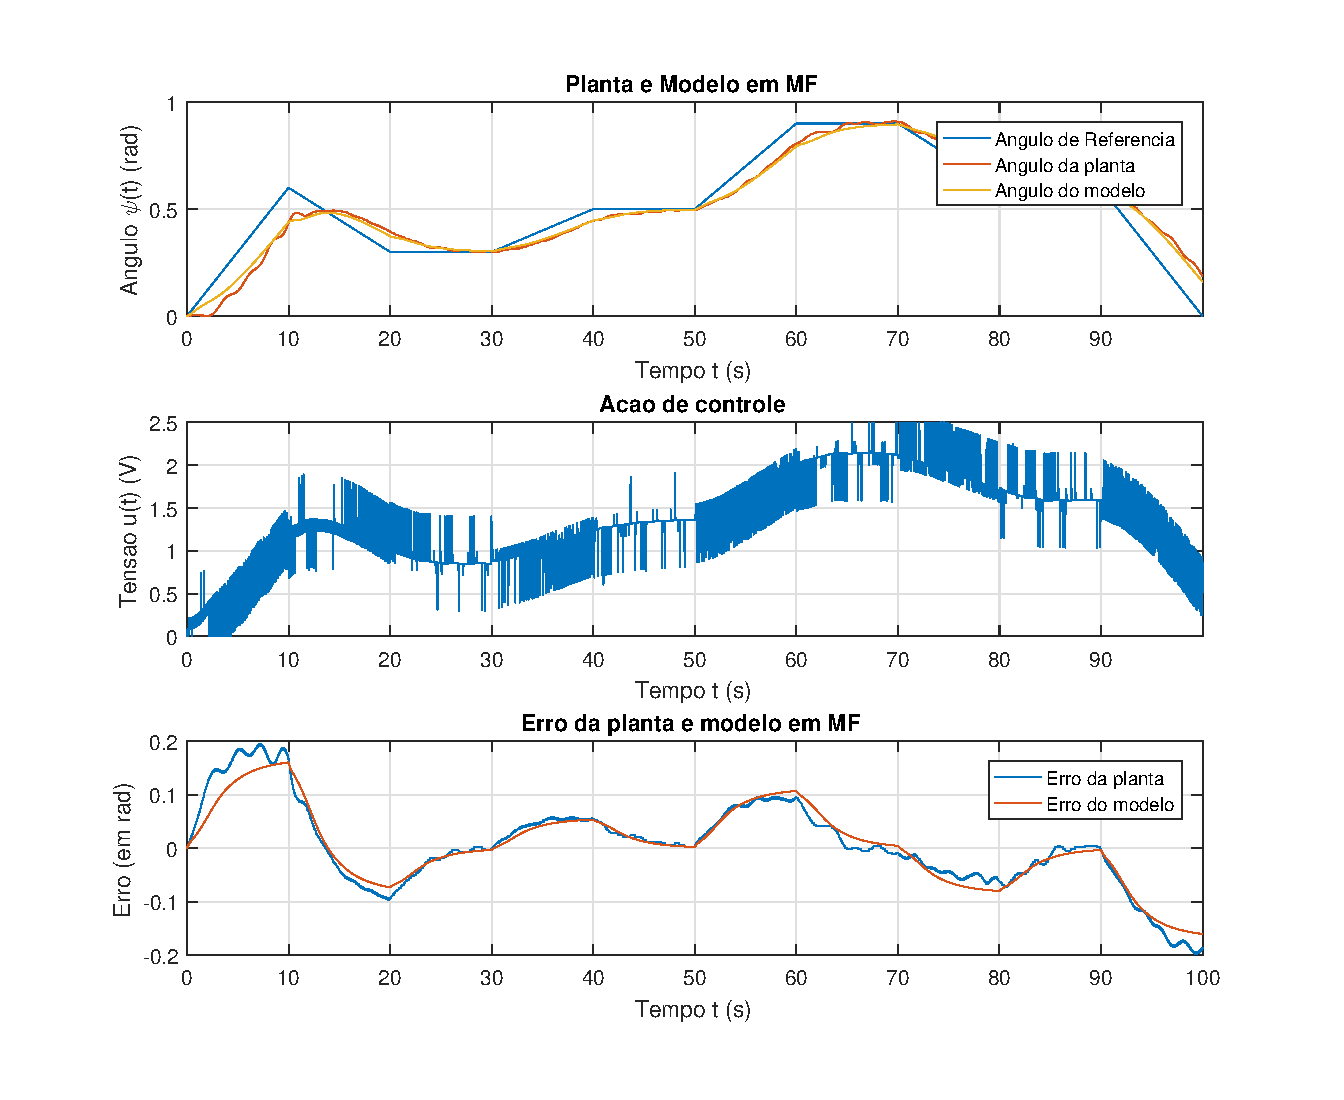
\includegraphics[width=0.5\textwidth]{figures/resultados/valida_pitch.eps}
    \caption{Validação de controle desacoplado de  \textit{pitch}.}
    \label{fig:ResultadosPitch}
\end{figure}

\begin{figure}[H]
    \centering
    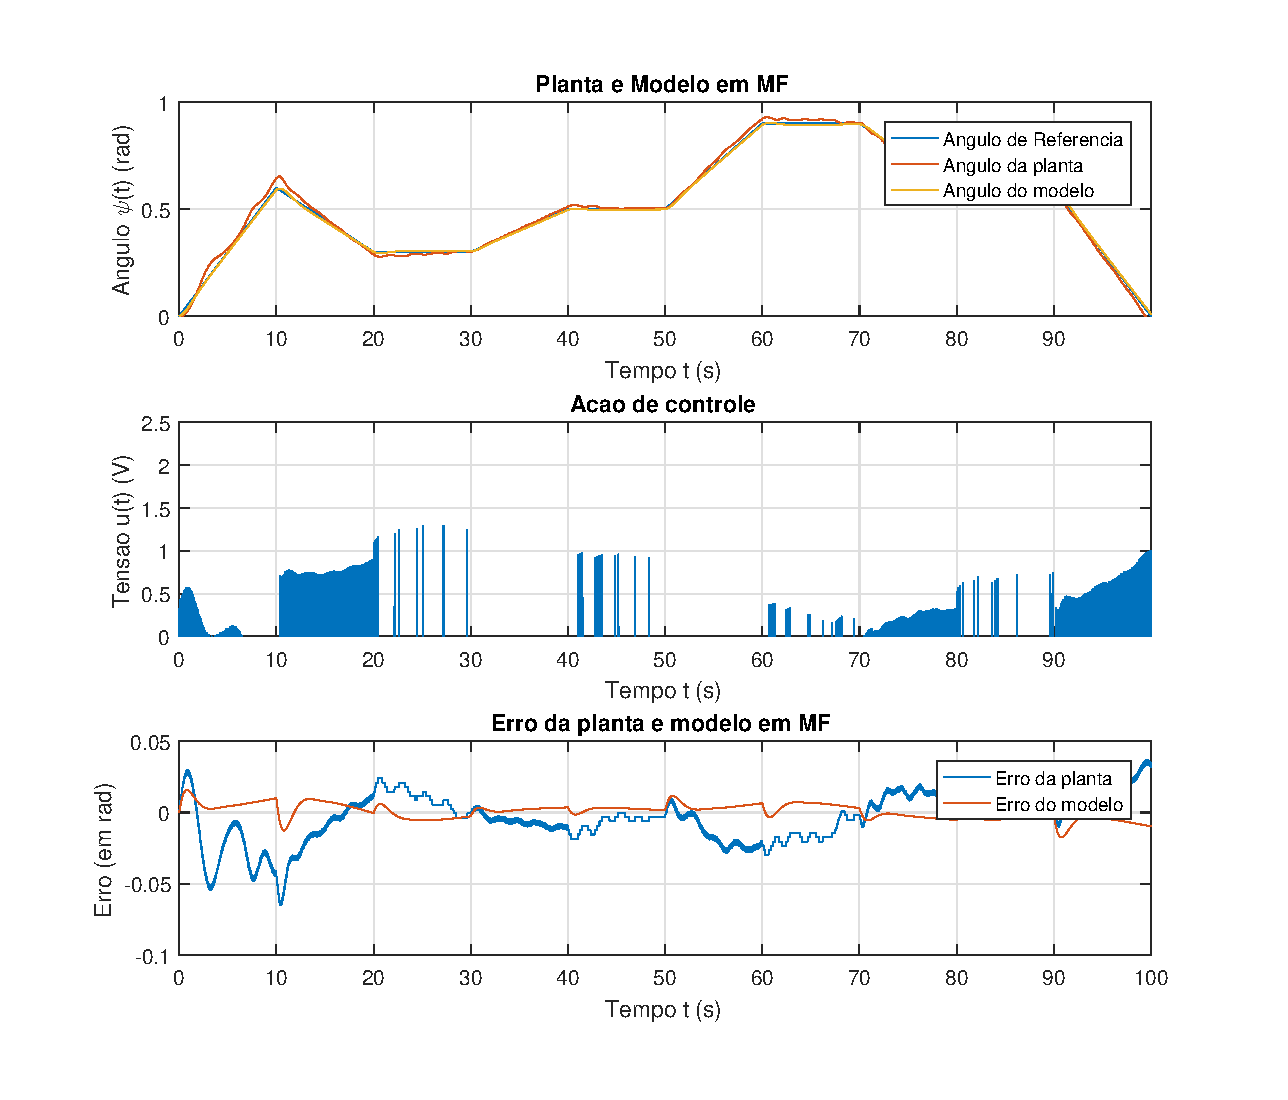
\includegraphics[width=0.5\textwidth]{figures/resultados/valida_yaw.eps}
    \caption{Validação de controle desacoplado de  \textit{yaw}.}
    \label{fig:ResultadosYaw}
\end{figure}


\subsection{\textbf{Análise de Desempenho}}

Para a avaliação de desempenho do sistema em malha fechada para a entrada variável mostrada na Figura \ref{fig:ValidaControladorEntradaVariavel}, foi realizada utilizando-se dois índices de desempenho, a Integral do Erro Quadrático (\textit{ISE - Integral Squared Error}) e a Integral do Erro Absoluto (\textit{IAE - Integral Absolute Error}). Os quais foram calculados por meio das equações \eqref{eq:ISE} e \eqref{eq:IEA}
 \begin{equation}\label{eq:ISE}
     ISE = \int_{0}^{T} e^{2}(t) dt
 \end{equation}
 \begin{equation}\label{eq:IEA}
     IEA = \int_{0}^{T} |e(t)| dt
 \end{equation}

\noindent onde $e$ é o erro, dado pela diferença entre o \textit{set-point} e o ângulo medido e $T$ representa a janela de tempo considerada.
 
Para o \textit{yaw}, obtivemos os seguintes índices:
$$ISE = 2.8430 $$
$$IAE = \SI{450.3624}{} $$
E para o \textit{pitch}, obtivemos:
$$ISE = 507.7020 $$
$$IAE = \SI{5.5331e+03}{} $$

